\subsubsection{28.01.15 (Соревнования)}
\begin{center}
	1-ый день соревнований "Робофест-Урал"
\end{center}
Сегодня проходила защита инженерных книг, оставшееся время было посвящено тренировкам и отладке автономного периода. На защите инженерной книги нас попросили рассказать защиту также на английском языке, с чем мы справились довольно посредственно. В целом, остальная защита прошла хорошо, но к следующим соревнованиям необходимо будет подготовить достойную защиту на английском. \newline
Внесенные доработки:
\begin{enumerate}
	\item Поскольку захват корзин в момент быстрого старта с места либо движения с максимальной скоростью часто открывался и робот терял подвижную корзину, было решено заменить сервопривод, приводящий в движение захват, на более мощный. Также были изменены откосы, центрующие корзину: они были перенесены выше для того, чтобы в том случае, когда захват закрывается неровно, откосы не цеплялись за бортики основания подвижной корзины. 
	\begin{figure}[H]
		\begin{minipage}[h]{0.47\linewidth}
			\center{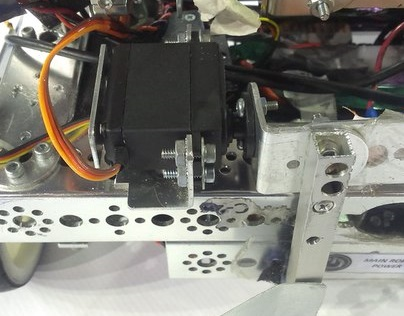
\includegraphics[scale=0.3]{days/28.01.15/images/01}}
			\caption{Замена сервопривода}
		\end{minipage}
		\hfill
	    \begin{minipage}[h]{0.47\linewidth}
	    	\center{
\includegraphics[scale=0.4]{days/28.01.15/images/02}}
	    	\caption{Замена откосов}
	    \end{minipage}
	\end{figure}
	
	\item Сегодня был реализован специальный держатель для флага альянса.
	\begin{figure}[H]
		\begin{minipage}[h]{0.47\linewidth}
			\center{
\includegraphics[scale=0.4]{days/28.01.15/images/03}}
		\end{minipage}
		\hfill
		\begin{minipage}[h]{0.47\linewidth}
			\center{
\includegraphics[scale=0.3]{days/28.01.15/images/04}}
		\end{minipage}
		\caption{Держатель флага}
	\end{figure}
	
	\item Из-за того, что новый захват мячей запускал мячи с большей скоростью, некоторые из них ударялись о верхний край ковша и падали обратно на лопатки, застопоривая их. Чтобы такого не происходило, мы приняли решение подрезать верхний край отверстия в передней части ковша. Кроме того, мы установили дополнительные пластины над захватом мячей, препятствующие выпадению мячей в том случае, если они все-таки будут подскакивать вверх.
	\begin{figure}[H]
		\begin{minipage}[h]{0.47\linewidth}
			\center{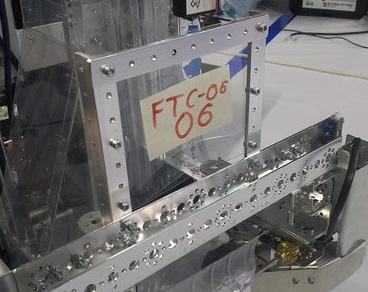
\includegraphics[scale=0.35]{days/28.01.15/images/05}}
			\caption{Дополнительные пластины}
		\end{minipage}
		\hfill
		\begin{minipage}[h]{0.47\linewidth}
			\center{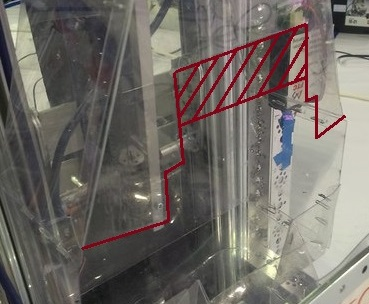
\includegraphics[scale=0.35]{days/28.01.15/images/06}}
			\caption{Ковш подрезан (заштрихована отрезанная область)}
		\end{minipage}
	\end{figure}
	
	\item Программа автономного периода для старта из зоны парковки была отлажена под характеристики поля. Программа автономного периода для старта сверху не была реализована, поскольку все остальные команды на соревнованиях имели программу старта с пандуса и мы решили не тратить на нее время на соревнованиях, а изготовить подвижную корзину (как минимум одну) дома и отладить эту программу дома.
	\begin{figure}[H]
		\begin{minipage}[h]{0.47\linewidth}
			\center{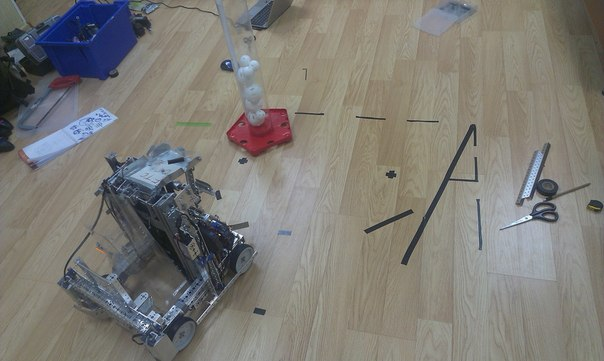
\includegraphics[scale=0.3]{days/28.01.15/images/07}}
		\end{minipage}
		\hfill
		\begin{minipage}[h]{0.47\linewidth}
			\center{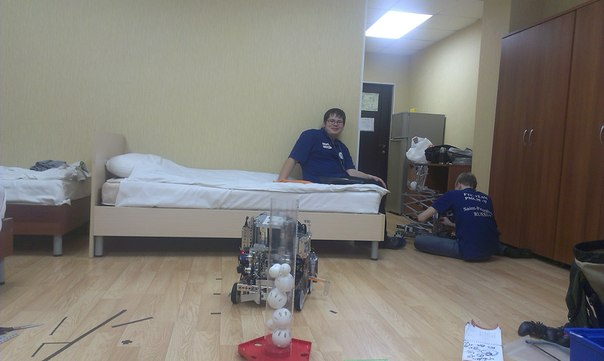
\includegraphics[scale=0.3]{days/28.01.15/images/08}}
		\end{minipage}
		\caption{Отладка программы в номере отеля}
	\end{figure}
	
\end{enumerate}
\fillpage